% Copyright 2004 by Till Tantau <tantau@users.sourceforge.net>.
%
% In principle, this file can be redistributed and/or modified under
% the terms of the GNU Public License, version 2.
%
% However, this file is supposed to be a template to be modified
% for your own needs. For this reason, if you use this file as a
% template and not specifically distribute it as part of a another
% package/program, I grant the extra permission to freely copy and
% modify this file as you see fit and even to delete this copyright
% notice. 

\documentclass{beamer}

% There are many different themes available for Beamer. A comprehensive
% list with examples is given here:
% http://deic.uab.es/~iblanes/beamer_gallery/index_by_theme.html
% You can uncomment the themes below if you would like to use a different
% one:
%\usetheme{AnnArbor}
%\usetheme{Antibes}
%\usetheme{Bergen}
%\usetheme{Berkeley}
%\usetheme{Berlin}
%\usetheme{Boadilla}
%\usetheme{boxes}
%\usetheme{CambridgeUS}
%\usetheme{Copenhagen}
%\usetheme{Darmstadt}
%\usetheme{default}
%\usetheme{Frankfurt}
%\usetheme{Goettingen}
%\usetheme{Hannover}
%\usetheme{Ilmenau}
%\usetheme{JuanLesPins}
%\usetheme{Luebeck}
\usetheme{Madrid}
%\usetheme{Malmoe}
%\usetheme{Marburg}
%\usetheme{Montpellier}
%\usetheme{PaloAlto}
%\usetheme{Pittsburgh}
%\usetheme{Rochester}
%\usetheme{Singapore}
%\usetheme{Szeged}
%\usetheme{Warsaw}

\usepackage[n,advantage, operators ,sets ,
        adversary,
        landau,
        probability,
        notions,
        ff,
        mm,
        primitives,
        events,
        complexity,
        asymptotics,
        keys,
        lambda]{cryptocode}
        
\newcommand{\scheme}{\mathsf{DD-Across}}
\newcommand{\msgspc}{\mathcal{M}}
\newcommand{\client}{\sigma_C}
\newcommand{\serv}{\sigma_S}
\newcommand{\smzero}{\textbf{m}_0}
\newcommand{\smone}{\textbf{m}_1}

\newcommand\blfootnote[1]{%
  \begingroup
  \renewcommand\thefootnote{}\footnote{#1}%
  \addtocounter{footnote}{-1}%
  \endgroup
}

\let\oldfootnotesize\footnotesize
\renewcommand*{\footnotesize}{\oldfootnotesize\tiny}


\setbeamersize{text margin left=1cm,text margin right=1cm} 


\title{Secure Deduplication Across Files}

% A subtitle is optional and this may be deleted
%\subtitle{Optional Subtitle}

\author{Nithin V Nath }
% - Give the names in the same order as the appear in the paper.
% - Use the \inst{?} command only if the authors have different
%   affiliation.


\institute[] % (optional, but mostly needed)
{
	Advisor: Dr. Bhavana Kanukurthi\\\vspace*{2mm}
	Department of Computer Science and Automation\\
	Indian Institute of Science
}
% - Use the \inst command only if there are several affiliations.
% - Keep it simple, no one is interested in your street address.

\date{23-Jun-2016}
% - Either use conference name or its abbreviation.
% - Not really informative to the audience, more for people (including
%   yourself) who are reading the slides online

\subject{Cryptography}
% This is only inserted into the PDF information catalog. Can be left
% out. 

% If you have a file called "university-logo-filename.xxx", where xxx
% is a graphic format that can be processed by latex or pdflatex,
% resp., then you can add a logo as follows:

% \pgfdeclareimage[height=0.5cm]{university-logo}{university-logo-filename}
% \logo{\pgfuseimage{university-logo}}

% Delete this, if you do not want the table of contents to pop up at
% the beginning of each subsection:
\AtBeginSubsection[]
{
  \begin{frame}<beamer>{Outline}
    \tableofcontents[currentsection,currentsubsection]
  \end{frame}
}

% Let's get started
\begin{document}

\begin{frame}
  \titlepage
\end{frame}

\begin{frame}{Outline}
  \tableofcontents
  % You might wish to add the option [pausesections]
\end{frame}

% Section and subsections will appear in the presentation overview
% and table of contents.
\section{Introduction}

\begin{frame}{Deduplication}{}
  \begin{itemize}
  \setlength\itemsep{1em}
  \item {
    Large amount of data stored in cloud storage.
  }
  \item {
    Multiple users store the same file.
  }
  \item {
    Service providers need to employ space saving techniques to keep cost down.
  }
	\begin{definition}
		Technique that enables storage providers to store a single copy of the data.
	\end{definition}
  \end{itemize}
\end{frame}

% You can reveal the parts of a slide one at a time
% with the \pause command:
\begin{frame}{Deduplication in Action}
  \begin{itemize}
  \setlength\itemsep{1em}
  \item {
    Alice uploads a file $M$ to the server $S$.
    %\pause % The slide will pause after showing the first item
  }
  \item {   
	 Bob requests to upload his copy of the same file $M$ to $S$.
  }
  % You can also specify when the content should appear
  % by using <n->:
  \item The server identifies
	that $M$ is already stored. 
   \item Server updates \textit{only the metadata} associated with $M$ to show
	that the file is owned by both Alice and Bob.
  %\item Make this an image
  \end{itemize}
\end{frame}

\subsection{Secure Deduplication}


\begin{frame}{Secure Deduplication}
\begin{itemize}
	\setlength\itemsep{1em}
	\item Deduplication along with privacy is a conflicting idea

	\item Users would like their data to be encrypted
	
	\item To enable deduplication, servers need to ``know the data"
\end{itemize}
\end{frame}

\begin{frame}{How to achieve Secure Deduplication}
	\begin{itemize}
		\setlength\itemsep{1em}
		\item \textbf{Key Idea}: Derive the key from the message itself.
		\item Generate a ``tag" from the ciphertext.
		\item Compare the tags of different ciphertexts to see if they are the same.
		\item We can achieve security only for unpredictable data.
	\end{itemize}
\end{frame}

\begin{frame}[allowframebreaks]{Motivation}
\begin{figure}
    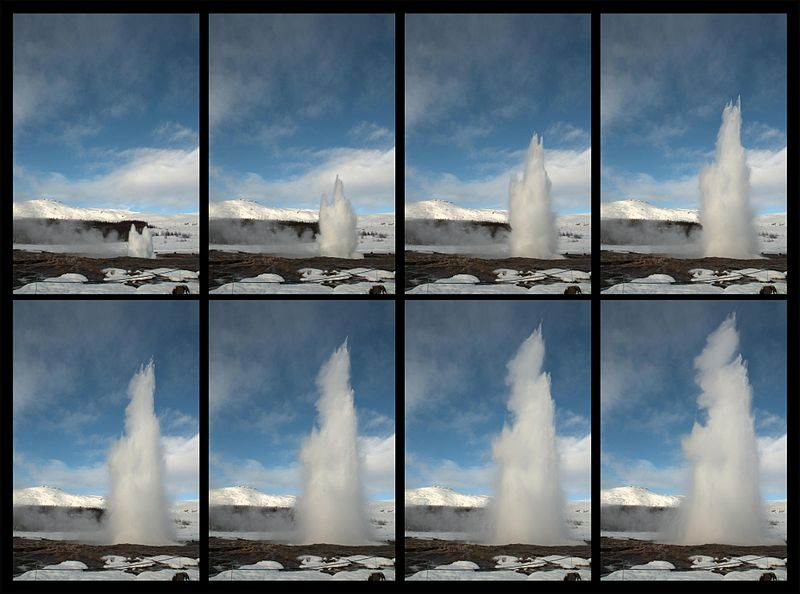
\includegraphics[scale=0.25]{burst.jpg}
\end{figure}
\begin{itemize}
	\setlength\itemsep{1em}
	\item Photos taken one after the other are often \textit{almost} identical to each other.\blfootnote{Photo courtesy: \url{https://commons.wikimedia.org/wiki/User:Papa_November}}
	\item These multiple files are not supported by existing file level deduplication.
	\item \textbf{Challenge}: Identify that plaintexts underneath these ciphertexts are 
		close to each other and store only the difference.
    \item \textbf{Problem Statement: }Achieve deduplication across files, which are close to each other, in a privacy preserving way.
\end{itemize}
\end{frame}

\subsection{Contribution}

\begin{frame}{Our Work}
	\begin{itemize}
		\setlength\itemsep{1em}
		\item $\scheme$ (deduplication across files) which enables deduplication even for files that are close to
	each other.
	    \begin{figure}[H]
	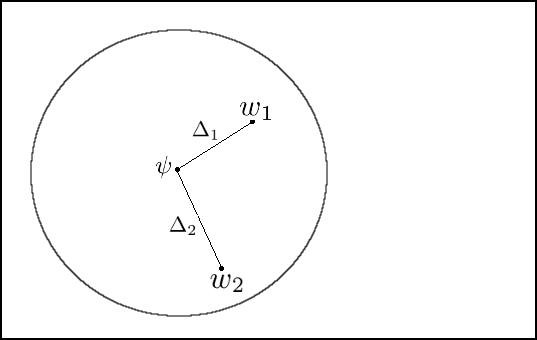
\includegraphics[scale=0.35]{example.png}
	%\caption{Rectangle box represents the entire message space. Only one of many balls is shown}
	\label{fig:example}
	\end{figure}
	\end{itemize}
\end{frame}

%\begin{frame}{Related Work}
%	\begin{itemize}
%		\setlength\itemsep{1em}
%		\item Convergent Encryption (year?)
%		\item Message Locked Encryption
%		\item Interactive Message Locked Encryption
%	\end{itemize}
%
%\end{frame}
%

%
%\begin{frame}{Message Locked Encryption}
%	\begin{itemize}
%		\setlength\itemsep{1em}
%		\item A cryptographic primitive. $\mathsf{MLE}=(\mathcal{P,K,E,D,T})$.
%		\item $\mathcal{K}_P(M)$ derives the key from the message.
%		\item $\mathcal{T}$ is the tag generation algorithm.
%		%\item Requires tag correctness and decryption correctness.
%		\item Semantic security cannot be achieved using MLE.
%		\item { [Include an image]}
%	\end{itemize}
%\end{frame}

\begin{frame}{Related Work - Interactive Message Locked Encryption}
	\begin{itemize}
		\setlength\itemsep{1em}
		%\item Extension of $MLE$.
		\item Uses interaction.
		\item Defined using one algorithm and three protocols
		\begin{enumerate}
		    \item $\mathsf{Init}(\secparam)$ - The initialization algorithm.
		    \item $\mathsf{Reg}$ - Register a client with the server.
		    \item $\mathsf{Put}(M, \client)$ - Puts a plaintext $M$ and returns $f$, an identifier
		    \item $\mathsf{Get}(f, \client)$ - Fetches the file $f$.
		\end{enumerate}
	\end{itemize}
\end{frame}

\subsection{Preliminaries}

\begin{frame}{Entropy}
	\begin{itemize}
		\setlength\itemsep{1em}
		\item Entropy is a measure of randomness
		\item Min-entropy of $X$ is the negative log of maximum predictability.
		\begin{equation*}
		    H_{\infty}(X) = - \log \left( \max\limits_{x} \mathsf{Pr} \left[ X=x \right] \right)
		\end{equation*}
		\begin{figure}
		    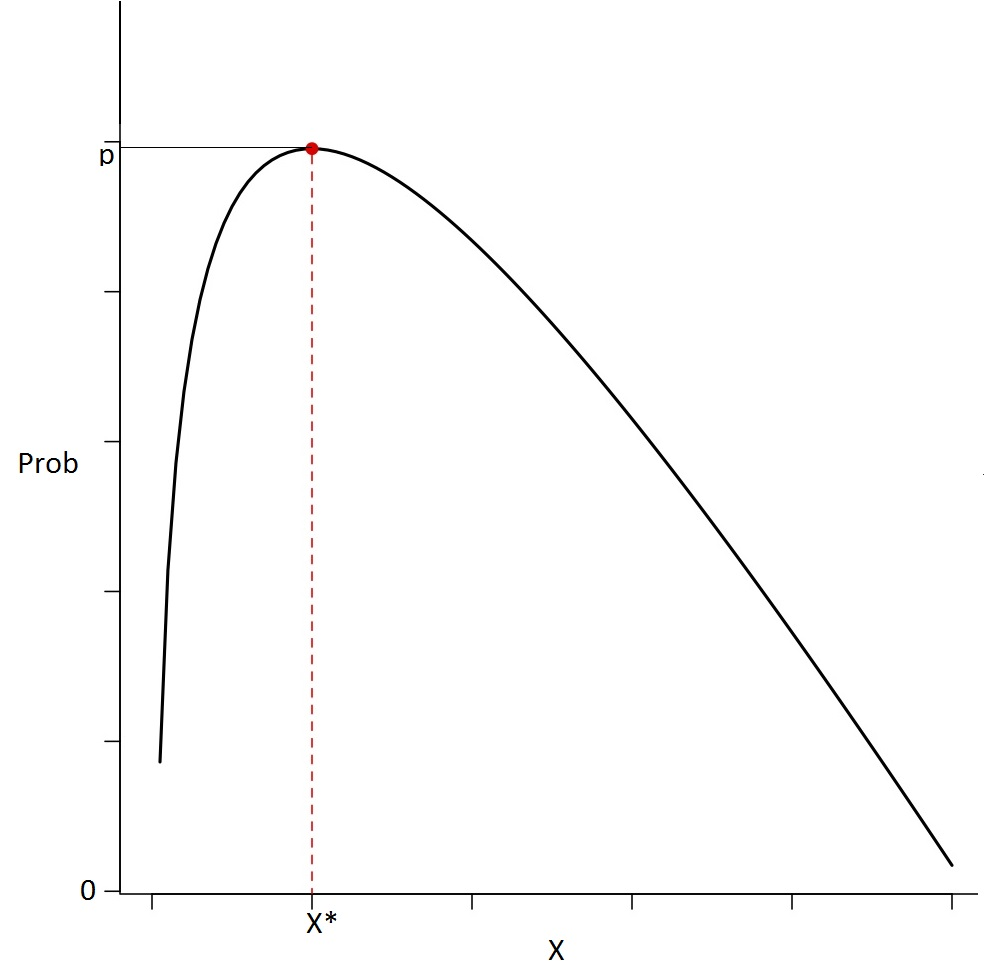
\includegraphics[scale=0.2]{min_entropy}
		\end{figure}
		\item Guessing Probability of $X$ is $GP(X)=2^{-H_{\infty}(X)}$
	\end{itemize}
\end{frame}

%\begin{frame}{Statistical Distance}
%	\begin{itemize}
%		\setlength\itemsep{1em}
%		\item 
%	\end{itemize}
%\end{frame}

\begin{frame}{Extractors}
	\begin{itemize}
		\setlength\itemsep{1em}
		\item A family of extractors $\ext = \{\ext_{\secpar}\}$
		\item $\ext_{\lambda} : \bin^{s(\secpar)} \times \bin^{l(\secpar)} \rightarrow \bin^{\kappa(\secpar)}$
		\begin{itemize}
		    \item $s$ - seed length
		    \item $l$ - input length 
		    \item $\kappa$ - output length
		\end{itemize}
		\item $(l,m,\kappa,\epsilon)$-strong extractor $\Rightarrow$ $\forall$ min-entropy  $m$ distributions $W$ on $\bin^l$
		    \begin{equation*}
		        \textbf{SD}\left(\left( \ext\left( W; X\right), X \right), \left( U_\kappa,X \right) \right) \leq \epsilon
		    \end{equation*}
		 where $X$ is uniform on $\bin^s$
	\end{itemize}
\end{frame}

\begin{frame}{Source}
	\begin{itemize}
		\setlength\itemsep{1em}
		\item The source S is an algorithm: $(\smzero, \smone) \leftarrow S(\secparam, d)$ where $d \in \bin^*$.
		\item $\smzero$ and $\smone$ are vectors over $\bin^*$
		%\item All components of the tuples $\smzero$ and $\smone$ are unique.
		\item $|\smzero| = |\smone|= m(\secpar)$.
		\item Guessing probability of source:
		    \begin{equation*}
                \textbf{GP}_\mathsf{S}(\secpar) = max_{i,b,d}\left( \textbf{GP}\left( \textbf{m}_b \left[ i \right] \right) \right)
            \end{equation*}
        \item We require $\textbf{GP}_\mathsf{S}(\secpar)$ to be negligible.
	\end{itemize}
\end{frame}

\begin{frame}{Deterministic Encryption}
	\begin{itemize}
		\setlength\itemsep{1em}
		\item $\mathsf{SE=(E, D)}$
		\item $c \leftarrow \mathsf{E}(\secparam, k, m)$
		\item $m \leftarrow \mathsf{D}(\secparam, k, c)$
		\item \textbf{Correctness:}  $\mathsf{D} \left( \secparam , k, \mathsf{E} \left( \secparam , k, m \right) \right) = m,\ \  \forall$  plaintexts $m \in \bin^*,\ \  \forall$  keys $k \in \bin^{\kappa(\lambda)},\ \   \forall \secpar \in \NN.$
	\end{itemize}
\end{frame}

\begin{frame}{Error Correcting Codes}
	\begin{itemize}
		\setlength\itemsep{1em}
		\item $(\msgspc, K, \tau)$-code $C$.
		\item $C$ is a subset $\{w_0, w_1, \ldots, w_K \}$ of $\msgspc$.
		\item $\tau > 0$ is the largest number such that there is at most one valid code word $c \in C$ for a message $w$ such that $\mathsf{dis}(w,c) \leq \tau$.
		\item $\mathsf{Enc}$ - The map from $i$ to $w_i$.
		\item $\mathsf{Dec}$ - The map that finds, given $w$, the $c \in C$ such that $\mathsf{dis}(w,c) \leq \tau$\
		
	\end{itemize}
\end{frame}

\begin{frame}{Collision Resistant Hash Functions}
	\begin{itemize}
		\setlength\itemsep{1em}
		\item $\mathcal{H}: \bin^n \rightarrow \bin^m$
		\item Collision resistant if 
		 \begin{itemize}
        \item $m < n$ and
        \item $\forall \ppt \adv$, $\exists$ a negligible function $\negl$ such that $\forall$ security parameters $\secpar \in \NN$,
            \begin{multline*}
            \mathsf{Pr} \left[ ( x_0, x_1) \leftarrow \adv \left( \secparam, \mathcal{H} \right): 
x_0 \neq x_1 \wedge \mathcal{H} \left( x_0 \right) = \mathcal{H}(x_1) \right] \leq \negl
            \end{multline*}
    \end{itemize}
        \item Family of hash functions: $\mathsf{H} = ( \mathcal{HK, H} )$
	\end{itemize}
\end{frame}



%\subsection{Road-map}
%\begin{frame}{Road-map}
%	\begin{itemize}
%		\setlength\itemsep{1em}
%		\item Setting
%		\item Adversarial Model
%		\item Privacy Games
%		\item $\scheme$ construction
%		\item $\scheme$ proof
%	\end{itemize}
%\end{frame}

\section{Construction}
\subsection{Adversarial Model}
\begin{frame}{Setting}
	\begin{itemize}
		\setlength\itemsep{1em}
		\item An honest-but-curious server.
		\item A set of clients.
		\item $\adv$ can control a subset of these clients.
		\item Formally modelled using a game $G$.
		\item $G$ sets up and controls an instance of a server.
		
	\end{itemize}
\end{frame}

\begin{frame}{Adversarial Model}
	\begin{itemize}
		\setlength\itemsep{1em}
        \item Adversary $\adv$ is invoked with oracle access to the following:\\
        \begin{itemize}
            \setlength\itemsep{1em}
            \item \textsc{Msg()}: allows adversary to set up multiple clients and to send arbitrary messages to the server.
            \item \textsc{Init()}: starts protocol instances on behalf of a legitimate client $L$, using inputs chosen by $A$.
            \item \textsc{Step()}: advances a  protocol instance by running the next step algorithm.
            \item \textsc{State()}: returns the server's state - including stored ciphertexts, public parameters, etc.
        \end{itemize}
    \end{itemize}
\end{frame}

\begin{frame}{The recovery game \textsc{Rec}}
    \begin{bbrenv}{A}
        \begin{bbrbox}[name=Adversary]
        \pseudocode{
            \\
            \textsc{Reg()} \text{ //Set up a legitimate client} \\
            \textsc{Init()} \\
            \textsc{Step()} \\
            \textsc{Msg()} \\
            \textsc{State()} \\
            win \leftarrow \textsc{WinCheck()}
        }
        \end{bbrbox}
        \bbroutput{$win$}
        \begin{bbrchallenger}{ChaA}
        \begin{bbrbox}[name=Challenger,minheight=2cm]
        \pseudocode{
            \\
            win \leftarrow False \\
            \sigma_S \sample \mathsf{Init}(1^\lambda)
        }
        \end{bbrbox}
        \end{bbrchallenger}
\end{bbrenv}
        
\end{frame}

\begin{frame}{The privacy game \textsc{Priv}}
    \begin{bbrenv}{A}
        \begin{bbrbox}[name=Adversary]
        \pseudocode{
            \\
            \textsc{Reg()} \\
            \textsc{Put}(i) \\
            \textsc{Step()} \\
            \textsc{Msg()} \\
            \textsc{State()} \\
        }
        \end{bbrbox}
        \bbroutput{$b'$}
        \begin{bbrchallenger}{ChaA}
        \begin{bbrbox}[name=Challenger,minheight=2cm]
        \pseudocode{
            \\
            b \sample \bin \\
            \sigma_S \sample \mathsf{Init}(1^\lambda)\\
            (\smzero, \smone) \leftarrow S(\secparam, \epsilon)\\
            \text{Ret }b=b'
        }
        \end{bbrbox}
        \end{bbrchallenger}
\end{bbrenv}
        
\end{frame}

\subsection{DD-Across}

\begin{frame}{DD-Across Ingredients}
	\begin{itemize}
		\setlength\itemsep{1em}
		\item A metric space ($\msgspc$, $\mathsf{dis}$)  with hamming distance as the distance metric.
        \item An $(l,m,\kappa,\epsilon)$-strong extractor.
        \item An error-correcting code $C = (\msgspc, K, \tau)$.
        \item A collision resistant hash function family $\mathsf{H}=(\mathcal{HK, H})$.
        \item $\mathsf{SE = (E,D)}$ denotes a symmetric encryption scheme.
	\end{itemize}
\end{frame}

\begin{frame}{DD-Across Construction}
	\begin{itemize}
		\setlength\itemsep{1em}
		\item $\scheme [C, \mathsf{H}, \mathsf{SE}]$.
		\item Server maintains 3 tables
		\begin{itemize}
		\item $\textbf{fil}$: which contains the encryptions of the files uploaded by the clients.
		\item $\textbf{delt}$: which stores the $\Delta$.
		\item $\textbf{own}$: which stores the ownership information.
		\end{itemize}
	\end{itemize}
\end{frame}

\begin{frame}{DD-Across Construction - Init}
		\begin{figure}[H]
    \centering
    \fbox{
	\procedure{Init}{%
	    S \sample \bin^{s (\lambda)}\\
	    K_h \sample \mathcal{HK}(1^\lambda)\\
		p = (S||K_h)\\
		\textbf{U} \leftarrow \phi \\
		\textbf{fil} \leftarrow \phi ; \textbf{delt} \leftarrow \phi \\
		\textbf{own} \leftarrow \phi \\
		\text{Ret } \sigma_S = (p, \textbf{U}, \textbf{fil}, \textbf{delt}, \textbf{own})
	}}
	\end{figure}
\end{frame}

\begin{frame}{DD-Across Construction - Reg}
		\begin{figure}[H]
    \centering
    \fbox{
	\procedure[width=0.5\textwidth]{Reg}{%
		\textbf{Reg[1]($\epsilon$)} \> \> \textbf{Reg[2]($\sigma_{S}$)}\\
		%k \sample \bin^{\kappa (\lambda)} \> \> \\
		\>  \sendmessageright{top=$\epsilon$, width=2.5cm, length=2cm} \> u \sample \bin^{\lambda} \setminus \textbf{U} \\
		\> \> \textbf{U} \leftarrow \textbf{U} \cup \{u\}\\
		\> \sendmessageleft{top={$(u,p)$}, width=2.5cm, length=2cm} \> \\
		\text{Ret } \sigma_c = (u, p) \> \>
	}}
	\end{figure}
\end{frame}

\begin{frame}{DD-Across Construction - Put}
		\begin{figure}[H]
    \centering
    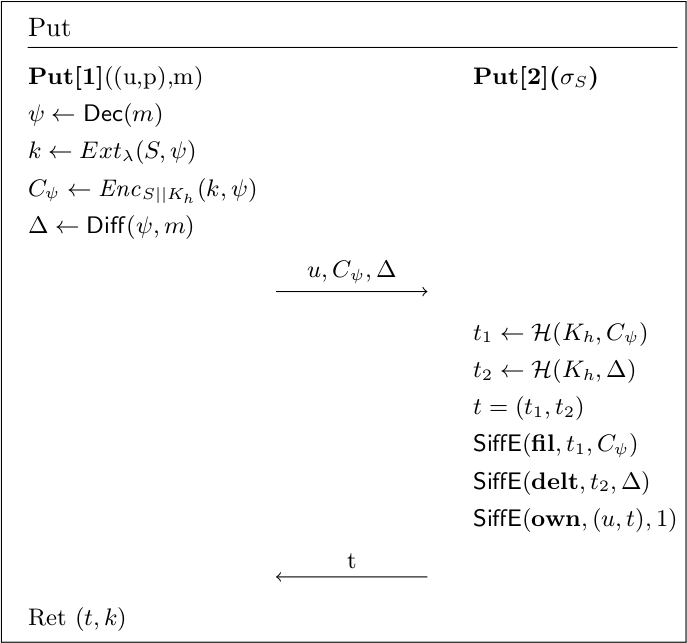
\includegraphics[scale=0.3]{put}
	\end{figure}
\end{frame}

\begin{frame}{DD-Across Construction - Get}
		\begin{figure}[H]
    \centering
    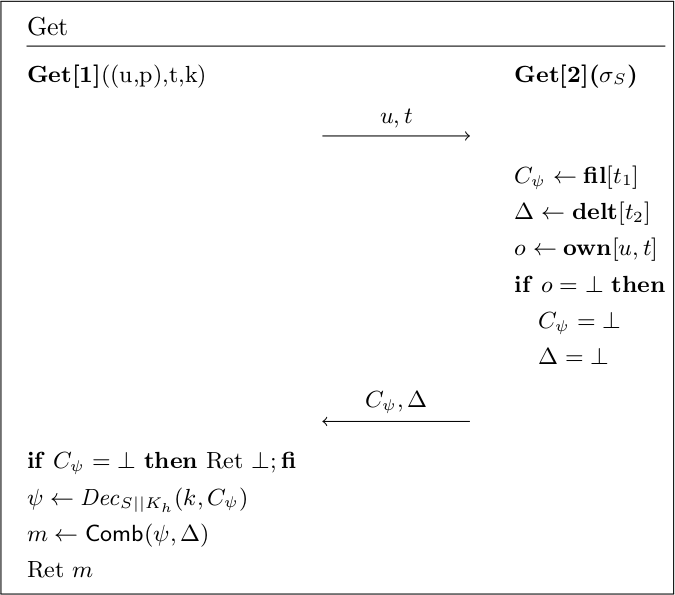
\includegraphics[scale=0.35]{get}
	\end{figure}
\end{frame}

\subsection{Recovery and Privacy}

\begin{frame}{DD-Across Recovery}
	\begin{itemize}
		\setlength\itemsep{1em}
		\item Recovery is guaranteed.
		\item For $\adv$ to ``win", $m_{\text{put}} \neq m_{\text{retrieved}}$ 
		\item Immutability of the tables means once put, file cannot be changed.
		\item Reduces to the security of hash collision.
	\end{itemize}
\end{frame}

\begin{frame}{DD-Across Privacy}

		\begin{definition}
        The error-correcting code $C=(\msgspc, K, \tau)$ is said to be compatible with a source $\mathsf{S}$ with min-entropy $\mu(\secpar)$ iff $2^{\mu(\secpar)-\tau}$ is negligible.
        \label{def}
        \end{definition}
        \begin{theorem}
    If $\mathcal{E}$ is CPA-secure and the code $C=(\msgspc, K, \tau)$ is compatible with the source $S$, then $\scheme_{RO}$[$\mathcal{E}$, $C$] \footnote{$\scheme_{RO}$ is the ROM analogue of $\scheme$ which models $\hash$ as a random oracle} is \textsc{Priv}-secure.
\end{theorem} 

\end{frame}

\begin{frame}{DD-Across Privacy Hybrids}
    \begin{figure}[H]
      \centering
      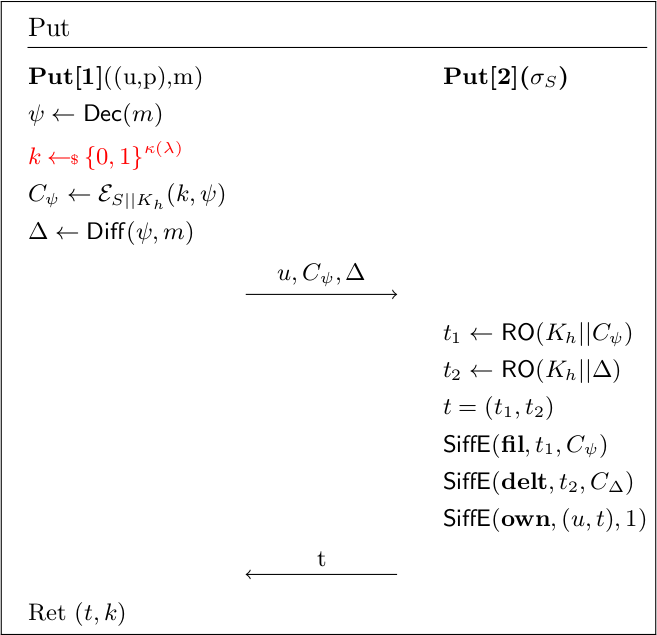
\includegraphics[scale=0.3]{H2}
      \caption{The $\mathsf{Put}$ protocol in game $H_2$}
    \end{figure}
\end{frame}

\begin{frame}{DD-Across Privacy Hybrids}
    \begin{figure}[H]
      \centering
      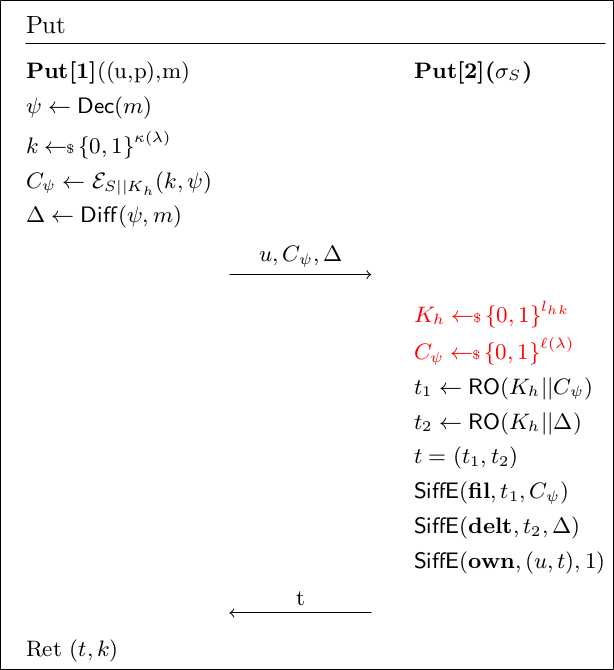
\includegraphics[scale=0.3]{H3}
      \caption{The $\mathsf{Put}$ protocol in game $H_3$}
    \end{figure}
\end{frame}

\begin{frame}{DD-Across Privacy Hybrids}
    \begin{figure}[H]
      \centering
      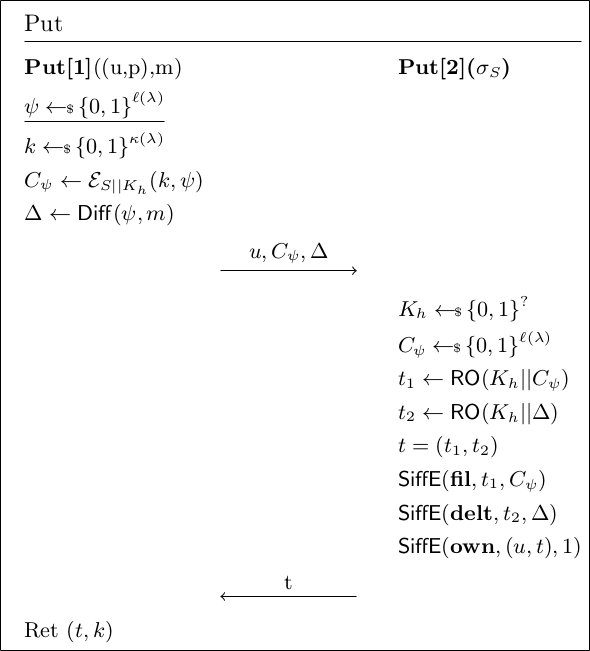
\includegraphics[scale=0.3]{H4}
      \caption{The $\mathsf{Put}$ protocol in game $H_4$}
    \end{figure}
\end{frame}

%\section{Conclusion}
%\begin{frame}{Summary}
%	\begin{itemize}
%		\setlength\itemsep{1em}
%		\item
%    
%  \item
%    Constructed a scheme called $\scheme$ that allows deduplication across files.
%  \item
%    Perhaps a \alert{third message}, but not more than that.
%	\end{itemize}
%\end{frame}
\section{Conclusion}
\begin{frame}{Open Problems and Future Work}
	\begin{itemize}
		\setlength\itemsep{1em}
		\item $\scheme$ allows deduplication across files when the files map to same code-word.
		%\item Connection of Fuzzy Extractors with the existing scheme.
		\item Implementing the scheme to record real world performance gains.
	\end{itemize}
\end{frame}


%\begin{frame}{Blocks}
%\begin{block}{Block Title}
%You can also highlight sections of your presentation in a block, with it's own title
%\end{block}
%\begin{theorem}
%There are separate environments for theorems, examples, definitions and proofs.
%\end{theorem}
%\begin{example}
%Here is an example of an example block.
%\end{example}
%\end{frame}

% Placing a * after \section means it will not show in the
% outline or table of contents.
%\section*{Summary}
%
%\begin{frame}{Summary}
%  \begin{itemize}
%  \item
%    The \alert{first main message} of your talk in one or two lines.
%  \item
%    The \alert{second main message} of your talk in one or two lines.
%  \item
%    Perhaps a \alert{third message}, but not more than that.
%  \end{itemize}
%  
%  \begin{itemize}
%  \item
%    Outlook
%    \begin{itemize}
%    \item
%      Something you haven't solved.
%    \item
%      Something else you haven't solved.
%    \end{itemize}
%  \end{itemize}
%\end{frame}



% All of the following is optional and typically not needed. 
\appendix
\section<presentation>*{\appendixname}
\subsection<presentation>*{For Further Reading}

\begin{frame}%[allowframebreaks]
  \frametitle<presentation>{For Further Reading}
    
  \begin{thebibliography}{10}
    
%  \beamertemplatebookbibitems
%  % Start with overview books.
%
%  \bibitem{Author1990}
%    A.~Author.
%    \newblock {\em Handbook of Everything}.
%    \newblock Some Press, 1990.
% 
    
  \beamertemplatearticlebibitems
  % Followed by interesting articles. Keep the list short. 

  \bibitem{MLE}
    Mihir Bellare, Sriram Keelveedhi, Thomas Ristenpart
    \newblock Message-Locked Encryption and Secure Deduplication.
    \newblock {\em Advances in Cryptology – EUROCRYPT}, 2013.
  
  \bibitem{iMLE}
    Mihir Bellare, Sriram Keelveedhi
    \newblock Interactive Message-Locked Encryption and Secure Deduplication.
    \newblock {\em Public Key Cryptography}, 2015.
  \end{thebibliography}
\end{frame}

\begin{frame}{}
\centering
	\fontsize{20pt}{7.2}\selectfont
	Thank You!
\end{frame}

\end{document}


\grid
